
\chapter{Multidimensional Visual Analysis (MVA)}

\label{chap:MVA}

Multidimensional Visual Analysis (MVA) refers to methods and
techniques to analyze and understand complex data sets using visual
representations. These approaches typically involve the use of
specialized software or tools that allow analysts to create and
manipulate graphical representations of the data in order to uncover
patterns, trends, and relationships. In this section, some popular MVA
approaches are reviewed \parencite{cao2011mva}.



\section{Scatter Plots}

A scatter plot is a type of graph that is used to display the
relationship between two numerical variables, to identify any
potential trends or patterns in the data, and to identify outliers. It
uses dots or markers to represent the values of the two variables, and
position of each dot on the graph indicates the value of the two
variables in a single observation.

To create a scatter plot, the values of one variable are plotted on the
x-axis (horizontal axis) and the values of the other variable are plotted
on the y-axis (vertical axis). The resulting graph will show a set of
dots, with each dot representing a single observation. If there is a
positive relationship between the two variables, the dots will tend to
form a diagonal line that slopes upwards from left to right. If there is a
negative relationship, the dots will tend to form a diagonal line that
slopes downwards from left to right. If there is no relationship between
the two variables, the dots will be scattered randomly across the graph.
Figure~\ref{fig:ScatterplotDiagram} shows an example of a scatter plot
displaying data point on x-axis and on y-axis

\begin{figure}[tp]
\centering
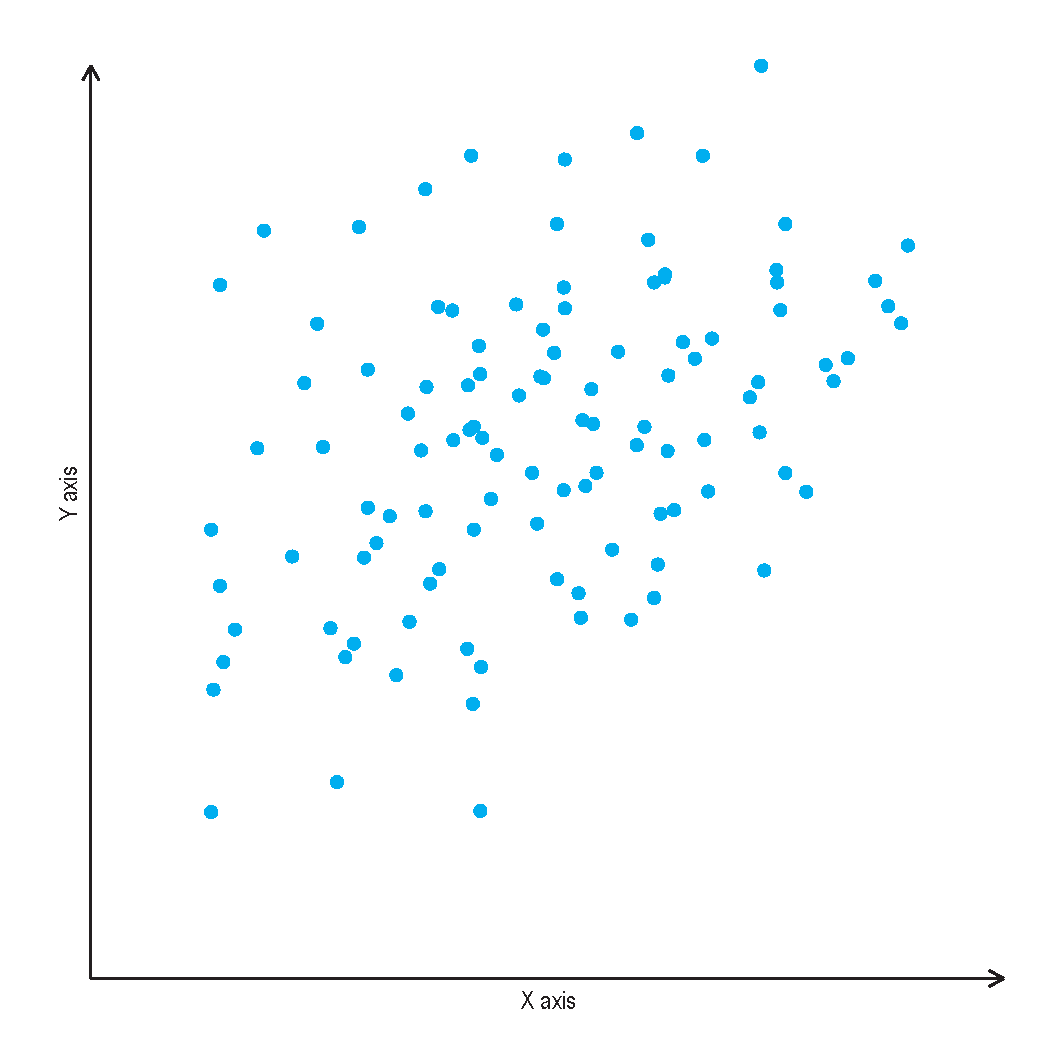
\includegraphics[frame,keepaspectratio,width=\linewidth,height=\halfh]
{diagrams/scatterplot.pdf}

\caption[Scatterplot]
{
A scatterplot displaying data points on x-axis and on y-axis.
\imgcredit{Drawn by Ožbej Golob.}
}
\label{fig:ScatterplotDiagram}
\end{figure}





\section{Similarity Maps}

Similarity maps are projections of high-dimensional datasets to two (or
sometimes three) dimensions. Projection techniques are used to reduce the
number of dimensions in the data, while attempting to preserve distances
between items as far as possible. Items which are close in the
high-dimensional space should also be close in the resulting
two-dimensional projection space. Such projections can be further split
into \emph{linear} and \emph{non-linear} projections.
Figure~\ref{fig:DimRed} shows an example visualization of data where
dimensions were reduced with the Principal Component Analysis (PCA). 

\begin{figure}[tp]
\centering
\subfloat[%  the % chars remove implicit spacing
The original 3-dimensional dataset. The red, blue, and green arrows are
the direction of the first, second, and third principal component,
respectively.
]
{%
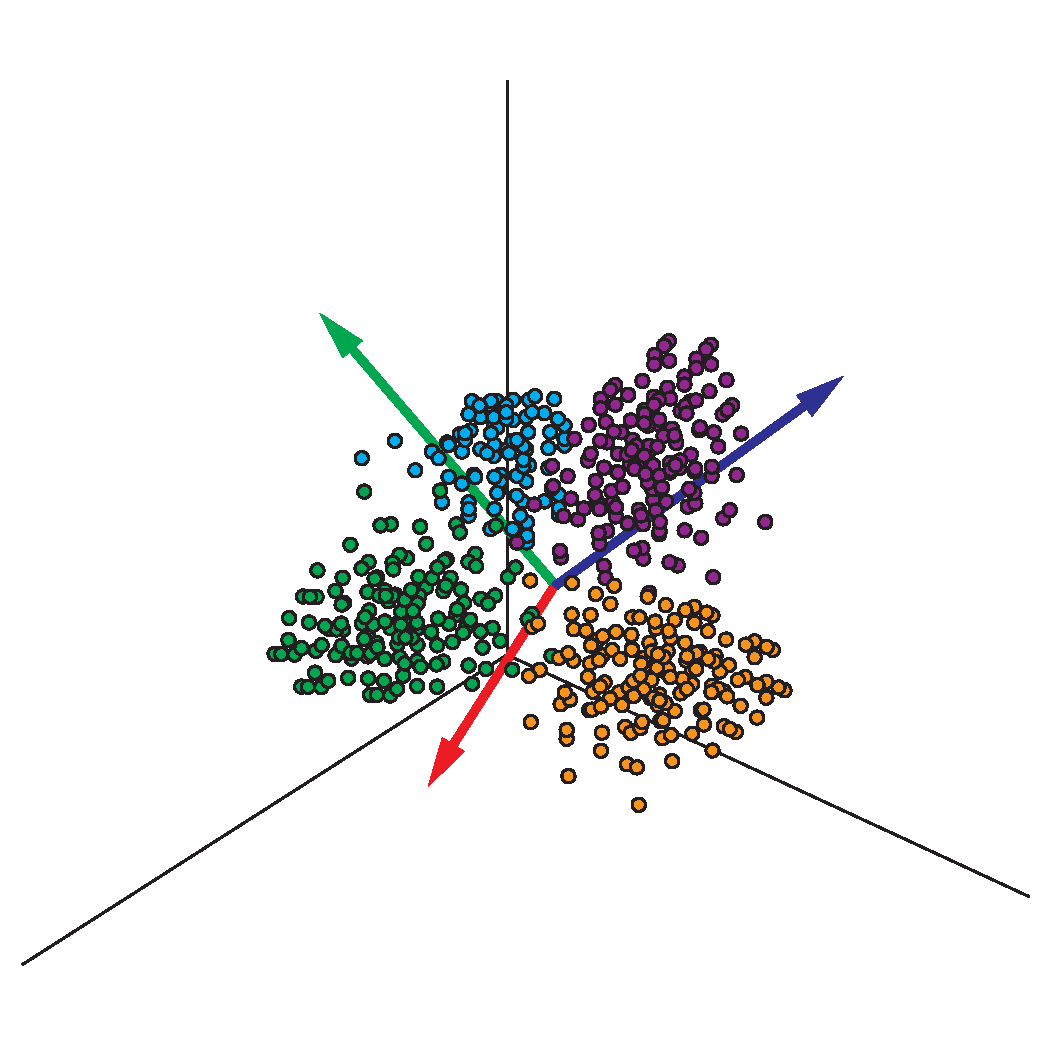
\includegraphics[valign=t,frame,scale=0.4]
{diagrams/pca-3d.pdf}%
\label{fig:DimRed3D}%
}
\hfill         % fills up the space between the two graphics
\subfloat[%
Scatter plot after PCA reduced from 3 dimensions to 2 dimensions.] {%
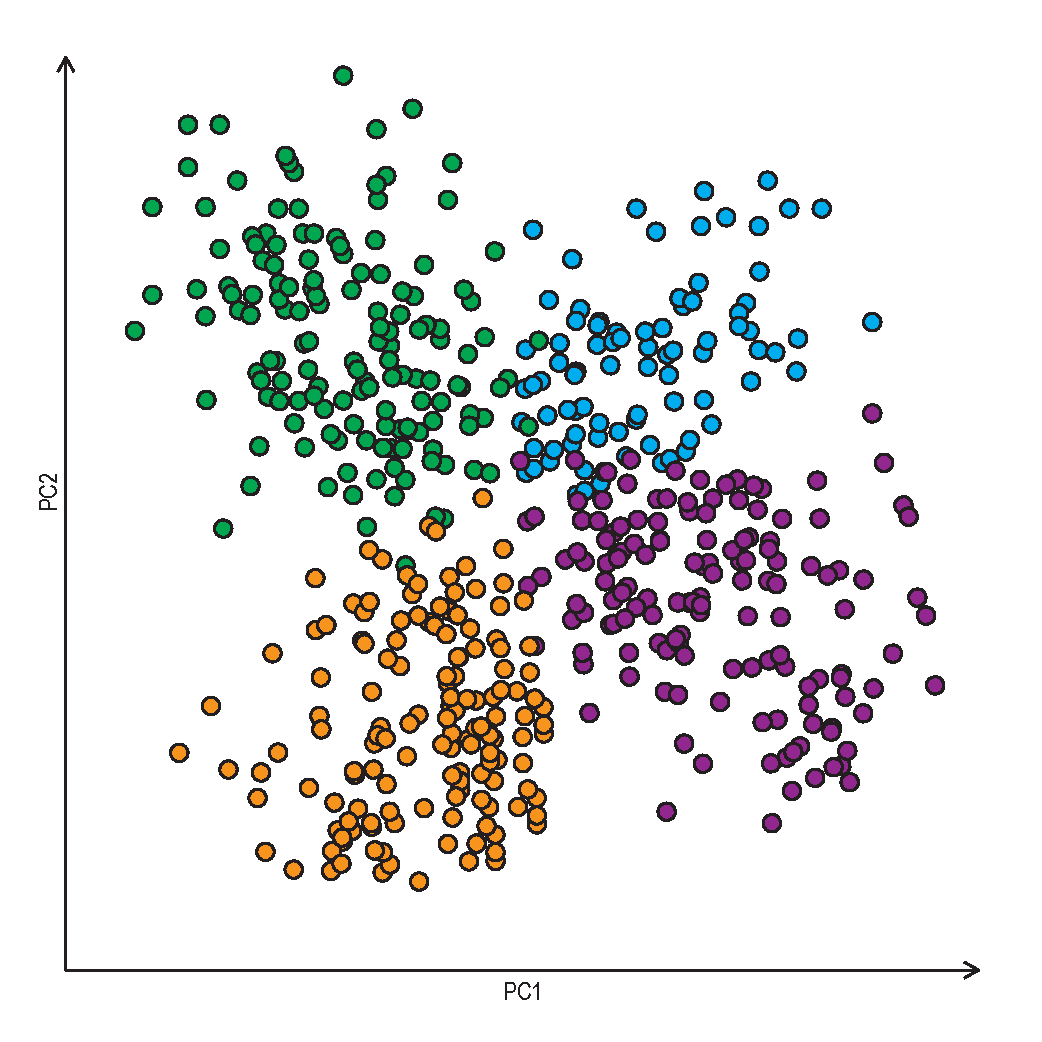
\includegraphics[valign=t,frame,scale=0.4]
{diagrams/pca-2d.pdf}%
\label{fig:DimRed2D}%
}

\caption[Dimensionality Reduction with PCA]
{Data visualisation before and after dimensionality reduction with the PCA
method.
\imgcredit{Both images created by Ožbej Golob.}
}
\label{fig:DimRed}
\end{figure}


\subsection{Principal Component Analysis (PCA)}

Principal Component Analysis (PCA) is a linear projection. PCA uses
linear algebra to identify the underlying dimensions or factors in the
data and project the data onto a lower-dimensional space
\parencite{abdi2010principal}.


\subsection{Multi-Dimensional Scaling (MDS)}

Multi-Dimensional Scaling (MDS) is a non-linear projection. MDS uses a
distance metric to preserve the distances between data points in the
high-dimensional space and project the data onto a lower-dimensional
space \parencite{morrison2003fast}.


\subsection{t-Distributed Stochastic Neighbor Embedding (t-SNE)}

t-Distributed Stochastic Neighbor Embedding (t-SNE) is a non-linear
projection. t-SNE uses a probabilistic model to preserve the local
structure of the data in the high-dimensional space and project the
data onto a lower-dimensional space \parencite{van2008visualizing}.


\subsection{Uniform Manifold Approximation and Projection (UMAP)}

Uniform Manifold Approximation and Projection (UMAP) is a non-linear
dimension reduction algorithm based on manifold learning techniques and
ideas from topological data analysis. UMAP is based on three assumptions
about the data: (i) The data has a uniform distribution of a Riemannian
manifold, (ii) The Riemannian metric is locally constant, and (iii) The
manifold is locally connected. UMAP uses these assumptions to model the
manifold with a fuzzy topological structure. The embedding is determined
by searching for a low-dimensional projection of the data that is the
closest equivalent to the fuzzy topological structure
\parencite{mcinnes2018umap}.




\section{Parallel Coordinates}

Parallel coordinates are a type of chart that is used to visualize
multi-dimensional data. In this type of chart, each data point is
represented by a vertical line that extends across multiple axes. The axes
are typically arranged in parallel. Each axis represents a different
variable, and the position of a point on that axis indicates the value of
that variable for the data point. This allows multiple variables to be
compared and analyzed simultaneously \parencite{inselberg1990parallel}.
Figure~\ref{fig:ParallelCoordinatesDiagram} shows an example of a parallel
coordinates plot displaying data points with multiple dimensions.

\begin{figure}[tp]
\centering
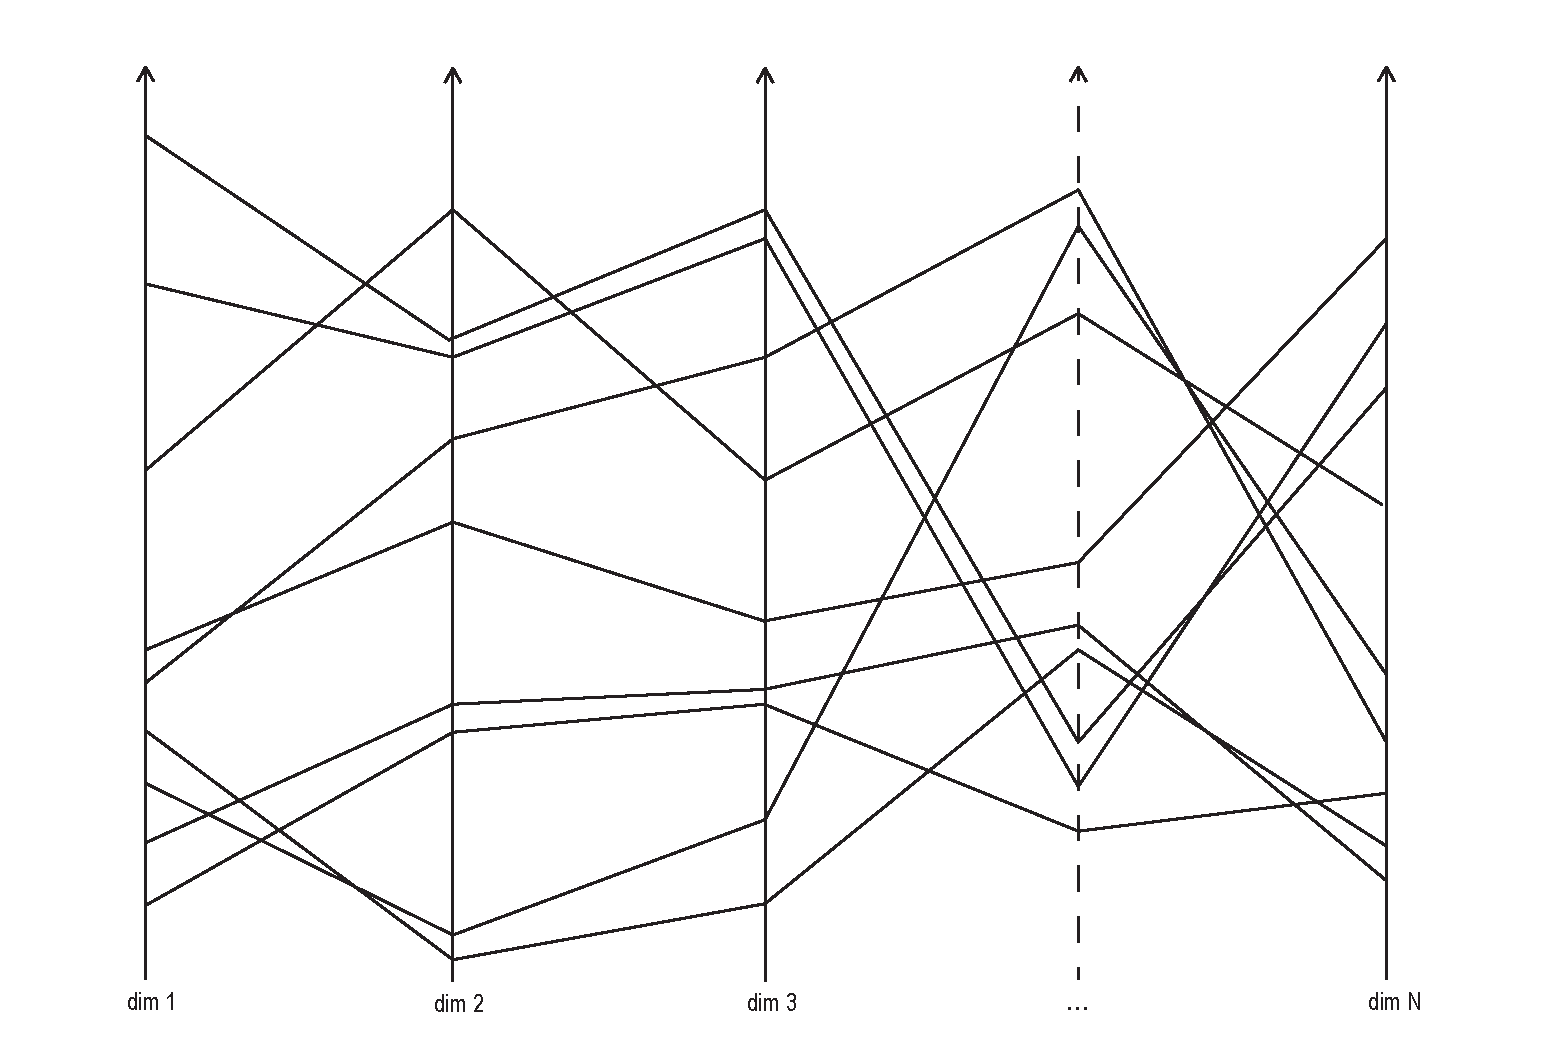
\includegraphics[frame,keepaspectratio,width=\linewidth,height=\halfh]
{diagrams/parallel-coordinates.pdf}

\caption[Parallel Coordinates]
{
A parallel coordinates plot displaying data points with multiple dimensions.
\imgcredit{Drawn by Ožbej Golob.}
}
\label{fig:ParallelCoordinatesDiagram}
\end{figure}






\section{Brushing and Linking}

Brushing and linking are techniques used in multidimensional visual
analysis to allow the user to interact with a visualization and
explore data in greater depth.

Brushing refers to the process of selecting data points or regions in one
visualization and highlighting those data points in other visualizations.
This allows the user to see how the data points or regions of interest are
related to other variables in the dataset.
Figure~\ref{fig:BrushingDiagram} shows an example of brushing. The user
selected a single data point which is now highlighted in all views with
red color.

Linking refers to the process of synchronizing the views of multiple
visualizations, such that a change made to one visualization is
reflected in the other visualizations. This allows the user to explore
the data from different perspectives and understand how different
variables are related to one another.

Both brushing and linking are useful for helping users to identify
patterns and relationships in the data and for facilitating the
process of data exploration and analysis.

\begin{figure}[tp]
\centering
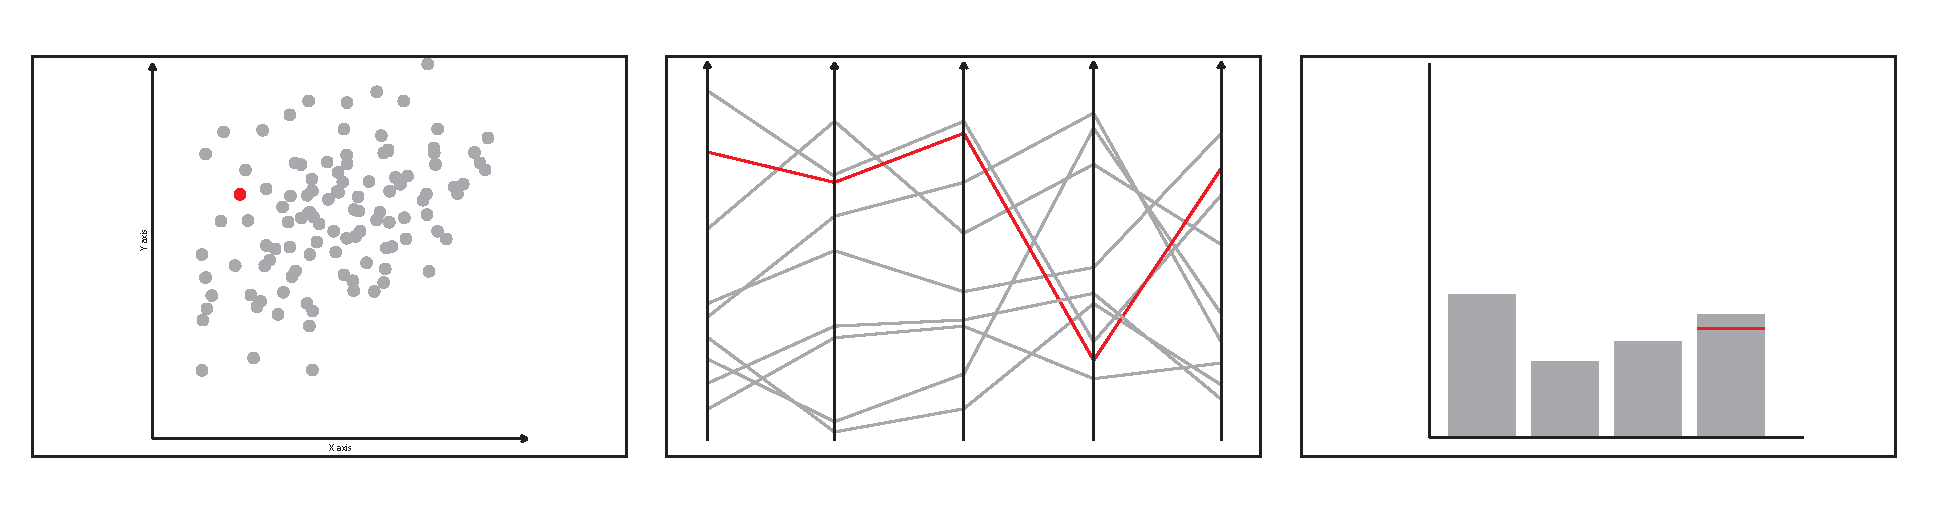
\includegraphics[frame,keepaspectratio,width=\linewidth,height=\halfh]
{diagrams/brushing.pdf}

\caption[Brushing]
{ An example of brushing. The user selected a single data point which
is now highlighted in all views with red color.
\imgcredit{Drawn by Ožbej Golob.}
}
\label{fig:BrushingDiagram}
\end{figure}




\section{Grouping and Labelling}

Grouping and labeling data is a fundamental step in the ML process.
Grouping refers to the process of identifying and separating similar data
points, while labeling refers to the process of providing relevant
information about the data. Grouping and labelling data helps to organize
and structure the data, making it easier to understand and work with. It
allows for more accurate and meaningful analysis of the data, as similar
data points can be grouped together and analyzed in relation to one
another. It also allows the ML model to understand the context of the data
and make more accurate predictions, and enables the interpretability of
the model, by providing meaningful information about the data and how it
is being used.

\subsection{Manual Grouping}

Manual grouping and labeling refers to the process of organizing and
providing relevant information about data manually, typically done by a
human. The process of manual grouping and labeling can be time-consuming
and labor-intensive.




\subsection{Automated Clustering}

Cluster analysis is a type of mathematical methods used to identify which
objects in a given data set are similar. It is a commonly used method for
exploratory data analysis, and is often used as a way to gain insight into
the underlying structure of the data. Cluster analysis methods sort
objects described as data. Objects with similar descriptions are grouped
into the same cluster. This allows analysts to identify common patterns
and trends within the data, and to gain a better understanding of the
relationships between the objects in the data set
\parencite{romesburg1984cluster}.



